\documentclass[a4paper]{article}

\usepackage[a4paper,top=2cm,bottom=2cm,left=0.5cm,right=0.5cm,marginparwidth=1.75cm]{geometry}
\usepackage[utf8]{inputenc}
\usepackage[english, russian]{babel}
\usepackage[]{amsmath,amsfonts,amssymb,amsthm,mathtools}
\usepackage[]{wasysym}
\usepackage[]{float}
\usepackage{multicol}
\usepackage{amsfonts}
\usepackage{indentfirst}
\usepackage{longtable}
\usepackage{natbib}
\usepackage{mathrsfs}
\usepackage{wrapfig}
\usepackage{graphicx}
\usepackage{mathtext}
\usepackage{amsmath}
\usepackage{siunitx} % Required for alignment
\usepackage{subfigure}
\usepackage{multirow}
\usepackage{rotating}
\usepackage[T1,T2A]{fontenc}
\usepackage{caption}
\usepackage{gensymb}


\date{\today}
\title{Лабораторная работа 3.2.3}
\author{Сидорчук Максим}

\begin{document}
\maketitle

\section{Цель работы}

Исследование резонанса токов в параллельном колебательном контуре с изменяемой ёмкостью, включающее получение амплитудно-частотных и фазово-частотных характеристик, а также определение основных параметров контура.

\section{В работе используются:}
Генератор сигналов, источник тока, колебательный контур с переменной ёмкостью, двулучевой осциллограф, цифровые вольтметры


\section{Теоретические положения}

Схема экспериментального стенда для изучения резонанса токов в параллельном колебательном контуре показана на рис. 1. Синусоидальный сигнал от генератора GFG-8255A поступает на вход источника тока, собранного на операционном усилителе ОУ с полевым транзистором ПТ, питание которых осуществляется встроенным блоком-выпрямителем от сети переменного тока 220 вольт. Цепи питания на схеме не показаны, представлен только резистор, переменное напряжение, на котором в используемой схеме равно напряжению на входе «+» операционного усилителя. \\

\begin{figure}[H]
    \centering
    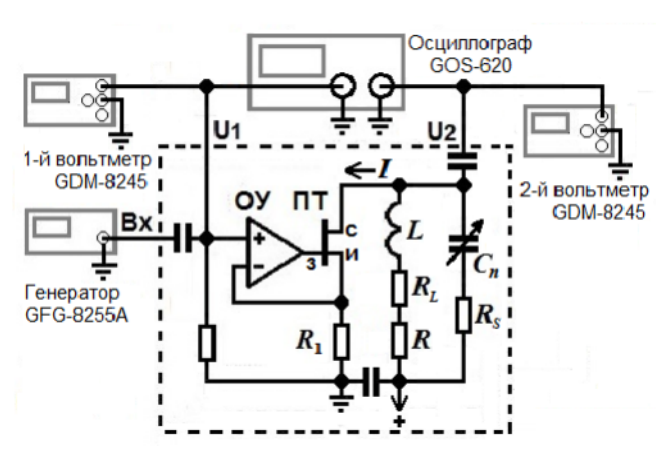
\includegraphics[width=10cm]{fig1.png}
    \caption{Схема экспериментального стенда}
    \label{fig:vac}
\end{figure}

Напряжение $ E = E_0cos(\omega t + \phi_0) $ поступает на вход «+» операционного усилителя от генератора через согласующую RC-цепочку. Это же напряжение через разъём «U1» подаётся одновременно на канал 1 осциллографа GOS-620 и вход 1-го цифрового вольтметра GDM-8245. Переменное напряжение на резисторе R1, как отмечалось выше, при этом также равно Е. Напряжение на контуре U, совпадающее с напряжением на конденсаторе, подаётся со знаком «–» через разъём «U2» на канал 2 осциллографа и вход 2-го цифрового вольтметра GDM-8245. Показанные на схеме установки ещё два конденсатора без наименований (помимо входящего в RC-цепочку) играют вспомогательную роль и не влияют на характеристики контура. Символ «->+» отмечает наличие источника питания полевого транзистора. Ток затвора «з» полевого транзистора ничтожно мал, так что токи истока «и» и стока «с» практически совпадают и равны току во внешней цепи контура. Как видно из схемы, \[ I = \frac{E}{R_1} = I_0cos(\omega t + \phi_0), \:\:\: I_0 = \frac{E_0}{R_1} \]

\section{Ход работы}

\subsection{Характеристики контура при разных емкостях}



Проведём измерения характеристик контура при разных значениях ёмкости конденсатора. Будем фиксировать резонансные частоты $f$ и напряжения $U$ в контуре при разных $C$, так же регистрируя входное напряжение $E$.

\begin{table}[h]
    \centering
    \begin{center}
        \caption{Измерения характеристик контура при разных ёмкостях}
    \end{center}
    \vspace{0.1cm}
    \label{tab:my_label}
    \begin{tabular}{ |c|c|c|c|c|c|c|c|c|c|c|}
        \hline
        $Cn,$ нФ                                            & $f,$ кГц & $U,$ В                 & $E,$ В & $L,$ мкГн & $\rho,$ Ом & $Z_\text{res},$ Ом & $Q$    & $R_{\Sigma},$Ом & $R_\text{max}, $Ом & $R_L$, Ом \\ \hline
        25.1                                                & 32       & 2                      & 0.4    & 985.522   & 198.151    & 5040               & 25.435 & 7.790           & 0.198              & 4.092     \\\hline
        33.2                                                & 27.8     & 1.6                    & 0.4    & 987.216   & 172.439    & 4032               & 23.382 & 7.374           & 0.172              & 3.702     \\\hline
        47.3                                                & 23.2     & 1.3                    & 0.4    & 994.954   & 145.034    & 3276               & 22.587 & 6.420           & 0.145              & 2.775     \\\hline
        57.4                                                & 21.1     & 1.1                    & 0.4    & 991.204   & 131.409    & 2772               & 21.094 & 6.229           & 0.131              & 2.598     \\\hline
        67.5                                                & 19.4     & 0.81                   & 0.4    & 997.086   & 121.538    & 2041.2             & 16.794 & 7.236           & 0.121              & 3.615     \\\hline
        82.7                                                & 17.6     & 0.63                   & 0.4    & 988.802   & 109.345    & 1587.6             & 14.519 & 7.531           & 0.109              & 3.921     \\\hline
        101.6                                               & 16       & 0.65                   & 0.4    & 973.882   & 97.905     & 1638               & 16.730 & 5.851           & 0.097              & 2.254     \\\hline
        \multicolumn{4}{|c|}{Среднее значение}              & 988.381  & \multicolumn{5}{|c|}{} & 3.279                                                                                                            \\ \hline
        \multicolumn{4}{|c|}{Среднеквадратичное отклонение} & 0.443    & \multicolumn{5}{|c|}{} & 0.0422                                                                                                           \\ \hline

    \end{tabular}
\end{table}

Для вычисления значений использовались формулы:\\
$$Z_\text{res} = \frac{U}{I_0} = \frac{U}{E/R_1}$$
$$\rho = \sqrt{\frac{L}{C}}$$
$$Q = \frac{Z_\text{res}}{\rho}$$
$$R_{\Sigma} = \frac{Z_\text{res}}{Q^2}$$
$$R_\text{smax} = \frac{tg\delta}{\omega C}$$
$$R_L = R_\text{smax} - R$$

\subsection{Нахождение АЧХ для с2 и с4}
Снимем амплитудно-частотную характеристику контура при ёмкостях $C_2$ и $C_4$. Для этого будем снимать зависимость напряжения в контуре от частоты колебаний.

\begin{table}[H]
    \centering
    \begin{center}
        \caption{Зависимость частоты колебаний от напряжения}
    \end{center}
    \vspace{0.1cm}
    \label{tab:my_label}
    \begin{tabular}{|c|c|c|c|}
        \hline
        \multicolumn{2}{|c|}{$C_2$} & \multicolumn{2}{c|}{$C_4$}                     \\
        \hline
        $f, $кГц                    & $U, $В                     & $f, $кГц & $U, $В \\
        \hline
        18                          & 0.039                      & 15       & 0.03   \\ \hline
        19                          & 0.04                       & 16       & 0.04   \\ \hline
        20                          & 0.05                       & 17       & 0.05   \\ \hline
        21                          & 0.06                       & 18       & 0.07   \\ \hline
        22                          & 0.07                       & 19       & 0.11   \\ \hline
        23                          & 0.09                       & 19.3     & 0.12   \\ \hline
        24                          & 0.11                       & 19.6     & 0.15   \\ \hline
        25                          & 0.16                       & 20       & 0.2    \\ \hline
        26                          & 0.24                       & 20.1     & 0.21   \\ \hline
        26.3                        & 0.28                       & 20.2     & 0.22   \\ \hline
        26.7                        & 0.37                       & 20.3     & 0.24   \\ \hline
        27.1                        & 0.512                      & 20.4     & 0.27   \\ \hline
        27.2                        & 0.576                      & 20.5     & 0.29   \\ \hline
        27.3                        & 0.649                      & 20.6     & 0.33   \\ \hline
        27.4                        & 0.68                       & 20.7     & 0.38   \\ \hline
        27.4                        & 0.73                       & 20.8     & 0.4    \\ \hline
        27.6                        & 0.91                       & 20.9     & 0.46   \\ \hline
        27.7                        & 0.87                       & 21       & 0.52   \\ \hline
        27.9                        & 0.89                       & 21.2     & 0.56   \\ \hline
        28                          & 0.85                       & 21.3     & 0.57   \\ \hline
        28.1                        & 0.79                       & 21.4     & 0.53   \\ \hline
        28.2                        & 0.74                       & 21.5     & 0.52   \\ \hline
        28.3                        & 0.69                       & 21.6     & 0.49   \\ \hline
        28.4                        & 0.62                       & 21.7     & 0.4    \\ \hline
        28.5                        & 0.56                       & 21.8     & 0.38   \\ \hline
        28.7                        & 0.45                       & 22       & 0.3    \\ \hline
        28.9                        & 0.41                       & 22.3     & 0.24   \\ \hline
        29                          & 0.36                       & 22.6     & 0.2    \\ \hline
        30.1                        & 0.21                       & 23       & 0.15   \\ \hline
        31                          & 0.15                       & 24       & 0.1    \\ \hline
        32                          & 0.12                       & 25       & 0.08   \\ \hline
        33                          & 0.1                        & 26       & 0.06   \\ \hline
        34                          & 0.08                       & 28       & 0.04   \\ \hline
        35                          & 0.07                       & 30       & 0.03   \\ \hline
        36                          & 0.06                       & 32       & 0.03   \\ \hline

    \end{tabular}
\end{table}

\begin{figure}[H]
    \centering
    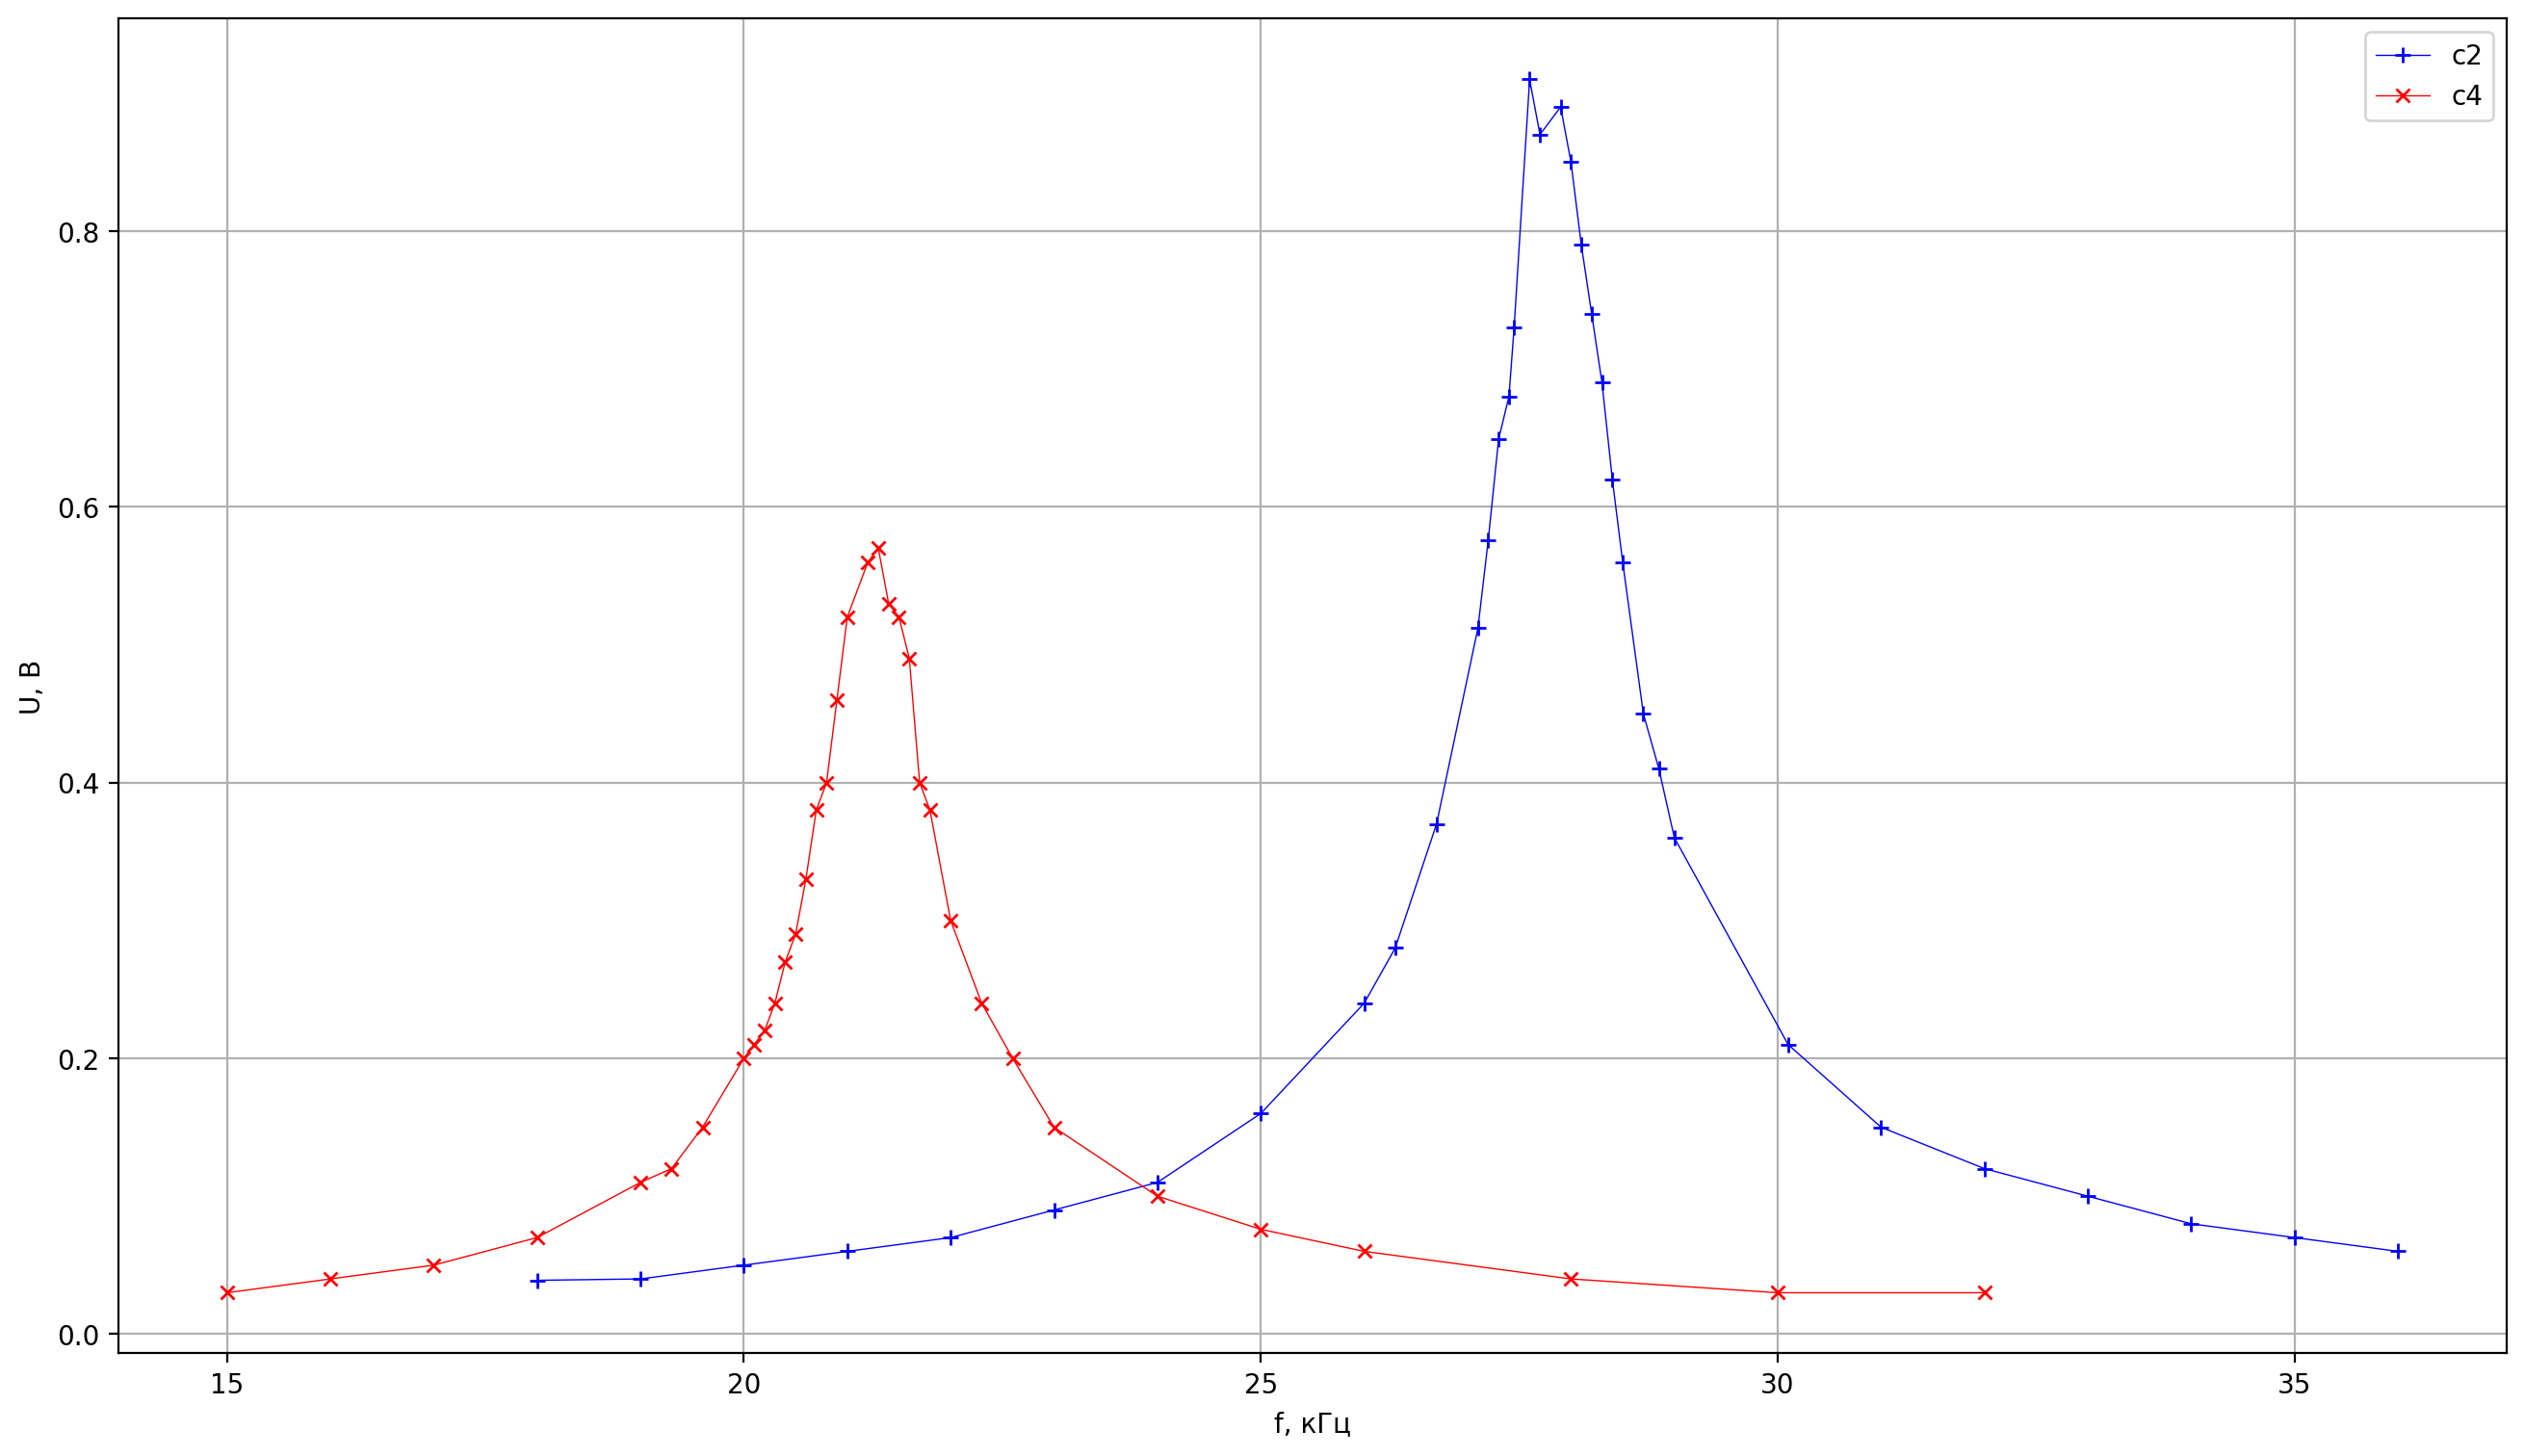
\includegraphics[width=\textwidth]{lol.png}
    \caption{АЧХ контуров с С2 и С4}
    \label{fig:vac}
\end{figure}

% Проведём сравнительный анализ АЧХ для двух ёмкостей в контуре. $C_4 > C_2$, формула для добротности $Q = \frac{1}{R}\sqrt{\frac{L}{C}}$. При повышении ёмкости падает добротность контура.

\subsection{АЧХ в относительных кооридинатах}

Построим графики АЧХ в координатах $U/U_0(f/f_0)$. По этим графикам (ширина резонансной кривой на уровне $\frac{1}{\sqrt{2}}$) определим добротность контуров: $Q_2 = 25.44$ и $Q_4 = 23.92$

Значения, определённые в пункте 1: $Q_2 = 23.38$ и $Q_4 = 21.09$

Полученные значения заметно различаются.

\begin{figure}[H]
    \centering
    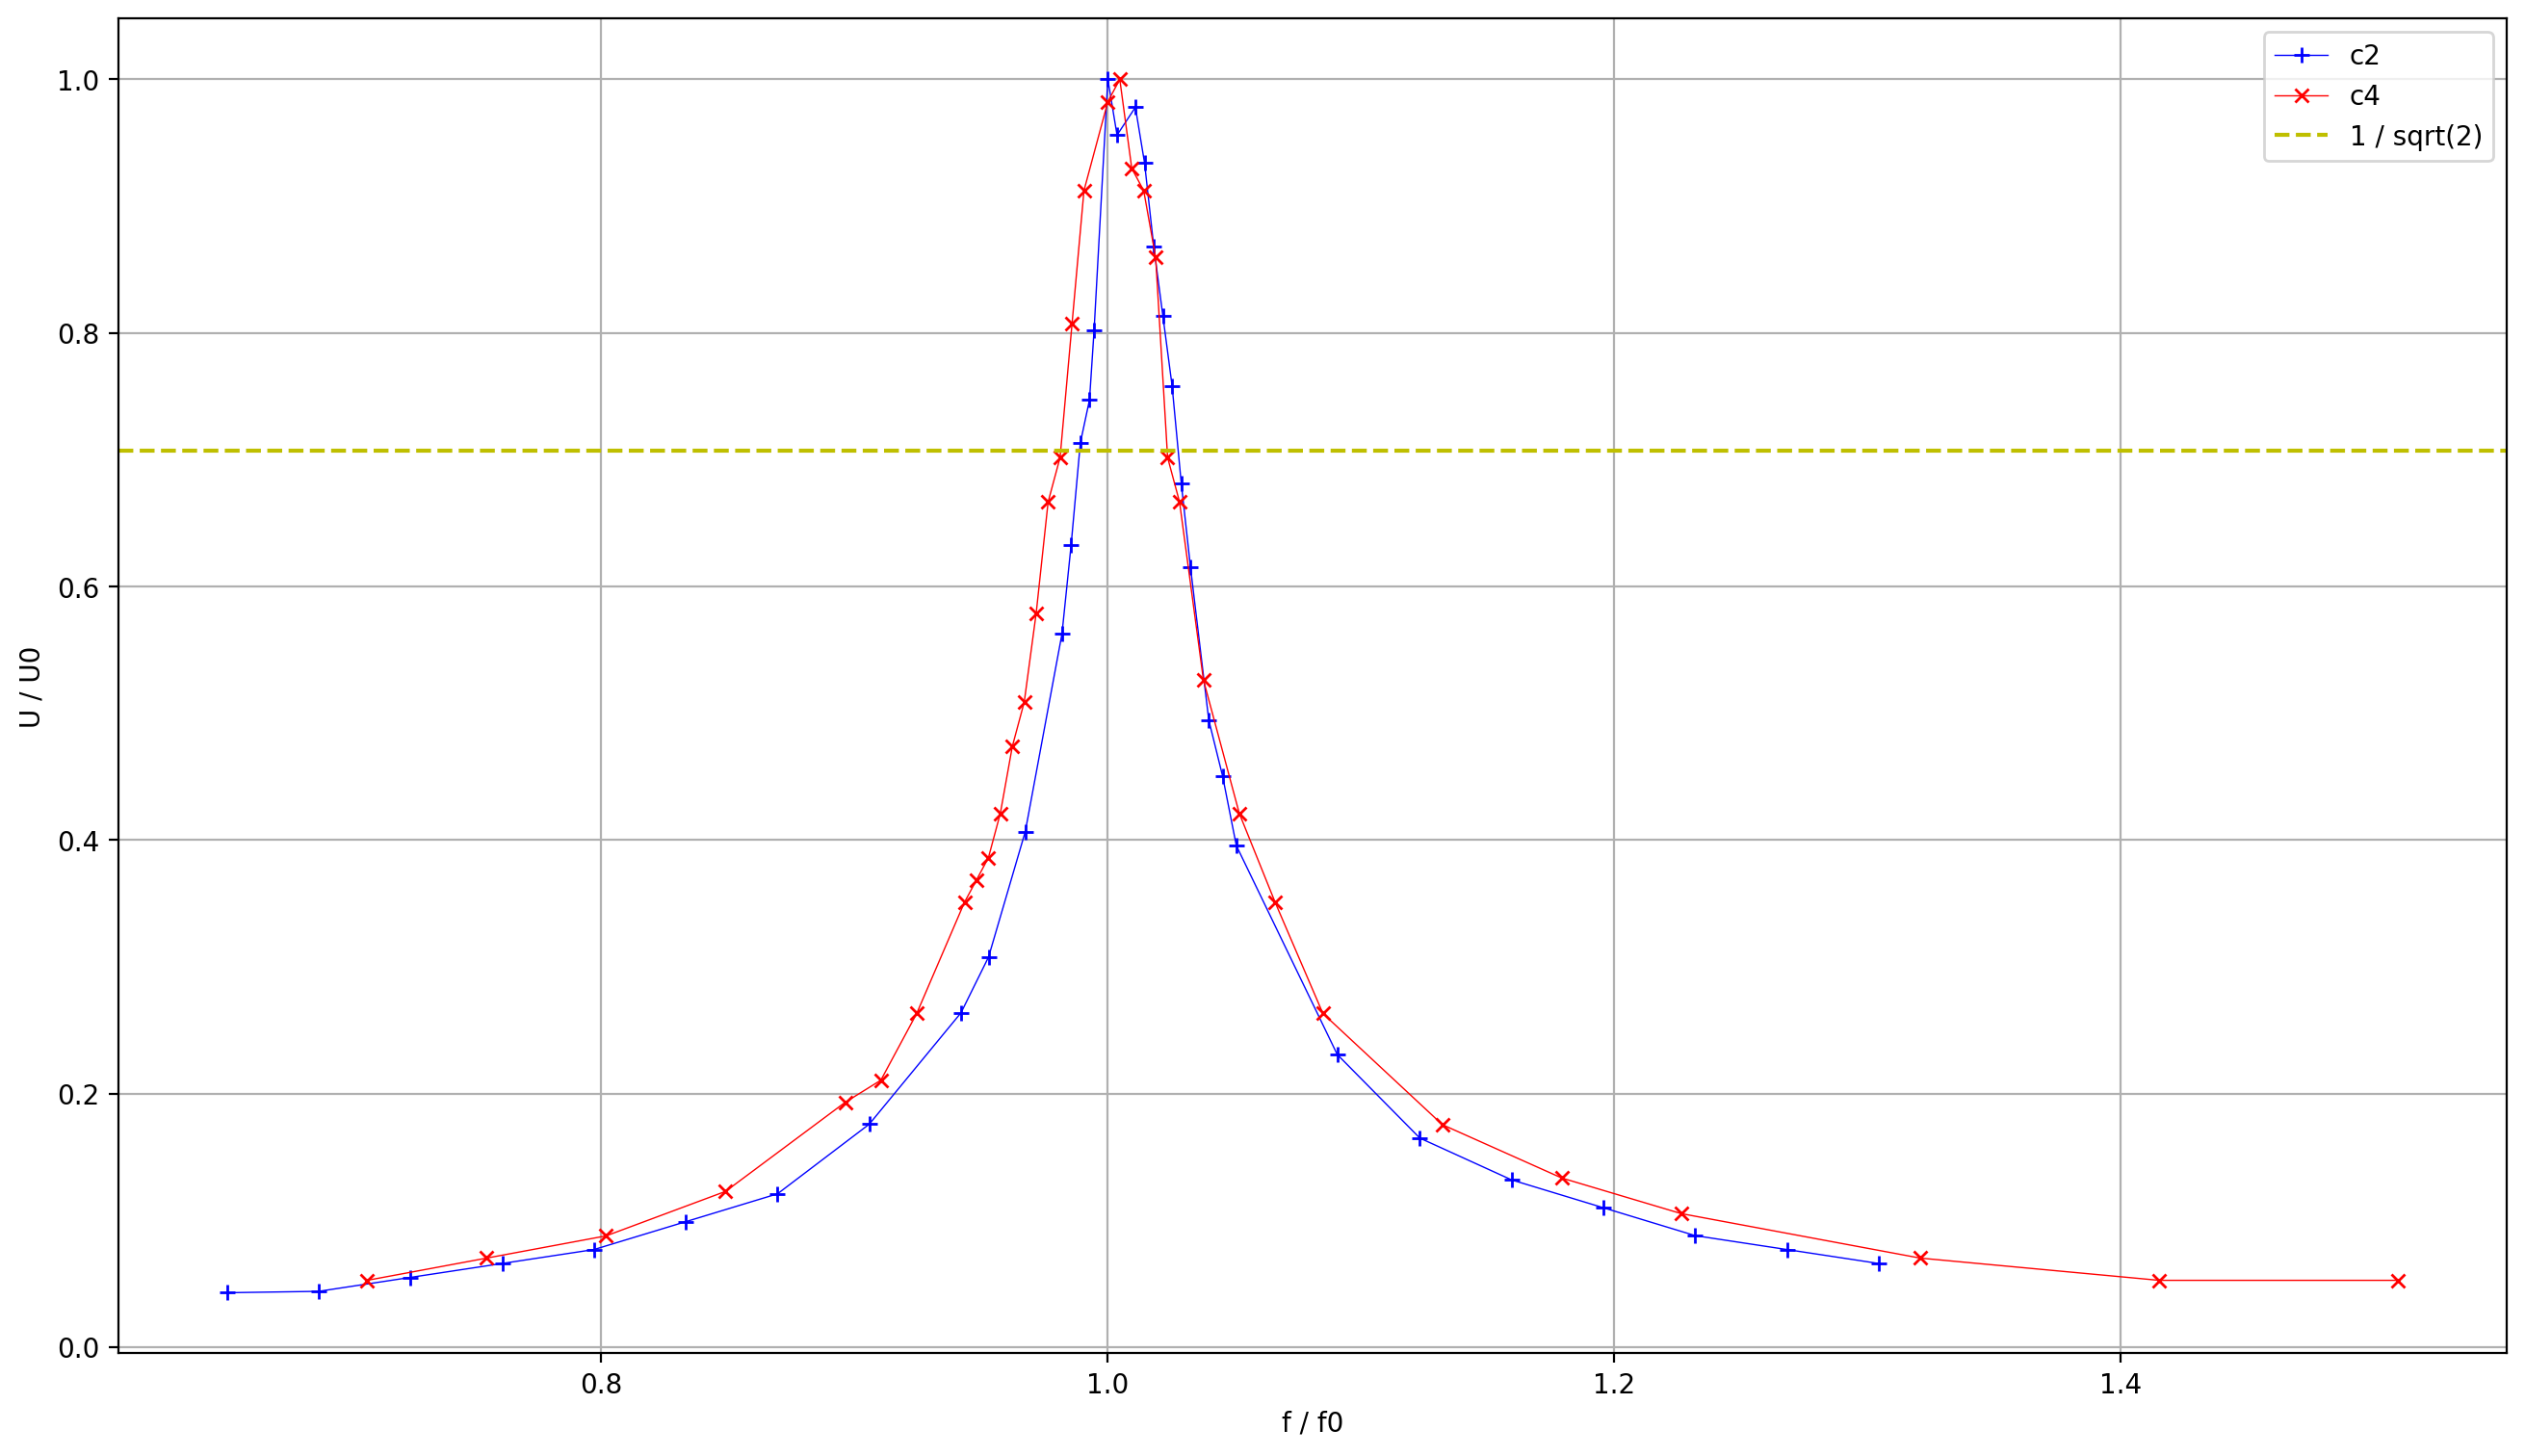
\includegraphics[width=\textwidth]{graph2.png}
    \caption{АЧХ контуров с С2 и С4 в относительных координатах}
    \label{fig:vac1}
\end{figure}

\subsection{ФЧХ}

Построим ФЧХ для контура с $C_2$ в координатах $x = f/f_0 \;\;\; y = \varphi/\pi   $ (рис. 4). По графику определим добротность контура следующим методом: расстояние между точками по оси $x$, в которых $y$ меняется от $-\pi/4$ до $\pi/4$, равно $1/Q$.

$$Q = \frac{1}{1.019-0.986} \approx 30.3$$

\begin{figure}[H]
    \centering
    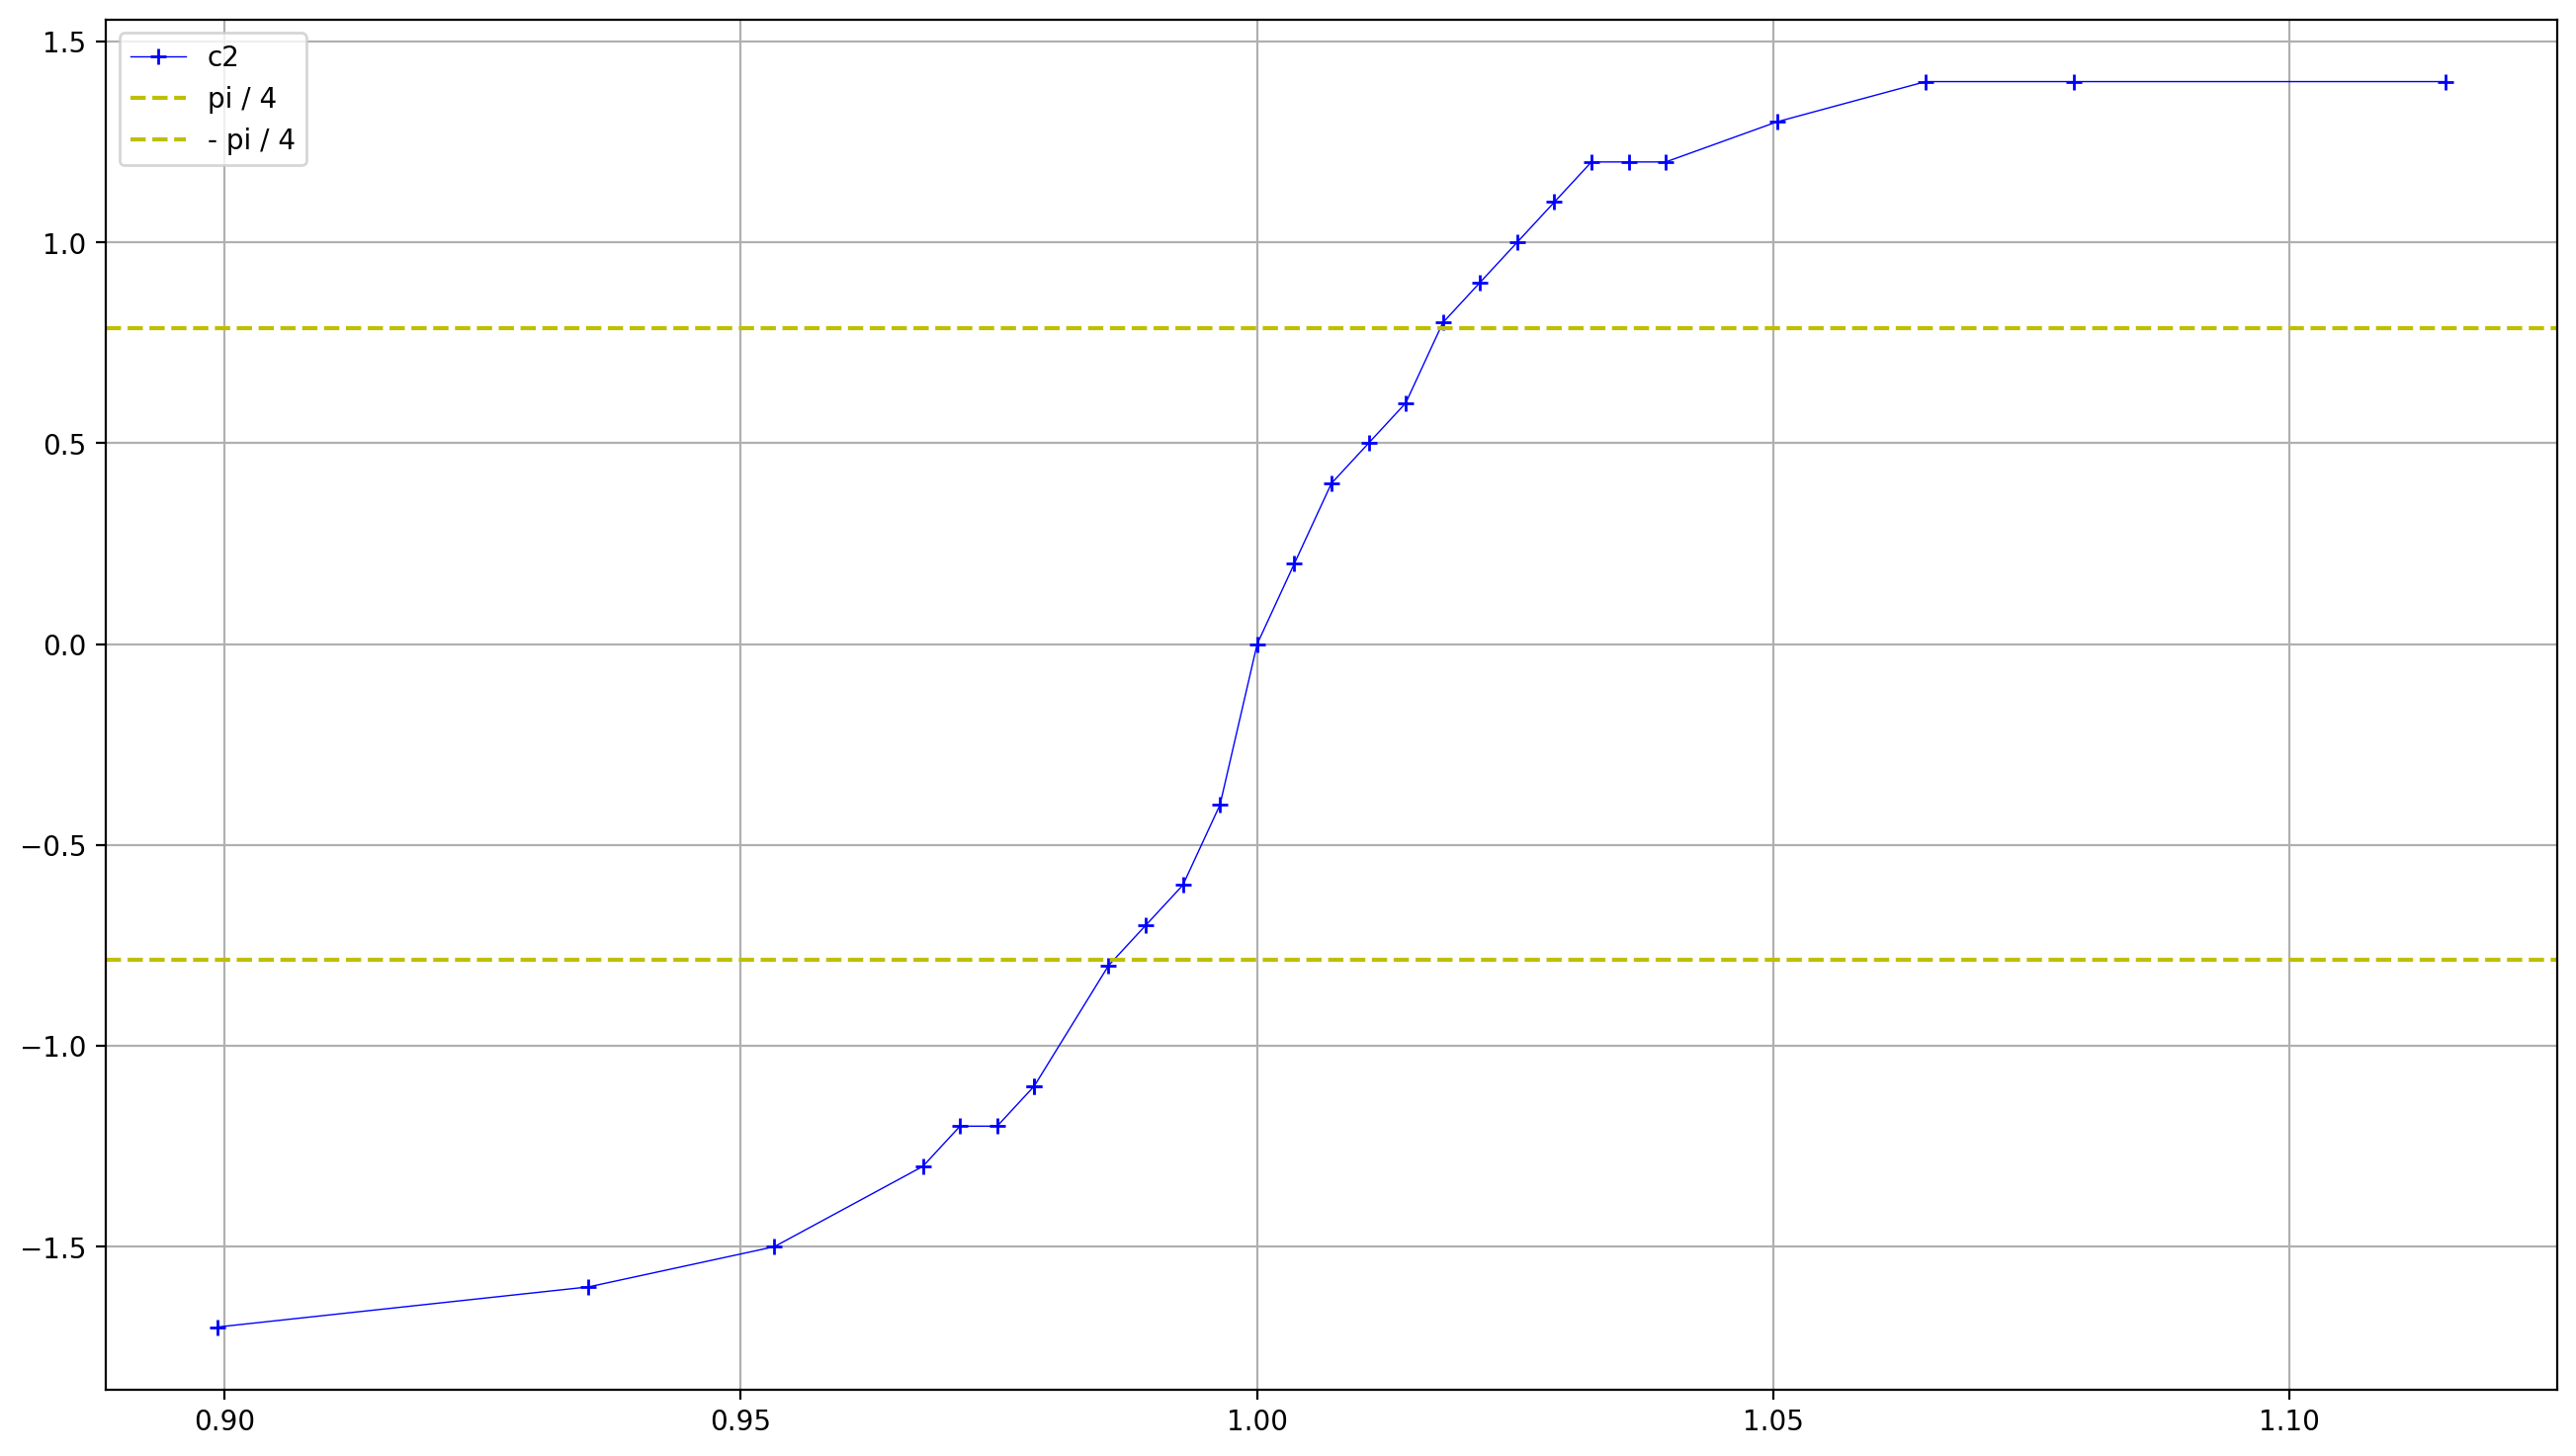
\includegraphics[width=\textwidth]{fchh.png}
    \caption{ФЧХ контура $C_2$}
    \label{fig:vac}
\end{figure}

\subsection{Векторная диаграмма}

Построим векторную диаграмму для токов и напряжений в последнем контуре (c7). Определим значения токов на конденсаторе и на катушке, а также напряжение в контуре по формулам
    $$I_0 = \frac{E}{R_1} = 0.0004 A$$
    $$I_c = I_L = Q I_0 = \frac{Q E}{R_1} = 0.007 A$$
    $$U = Q\rho I_0 = \frac{Q\rho E}{R_1} = 0.650B$$

Также определим сдвиги по фазе их от основного тока $I_0$:
    $$\varphi_c = \frac{\pi}{4} - \frac{R + R_L}{\rho} =  41^{\circ}$$
    $$\varphi_L = -\frac{\pi}{2} + \delta = -90 ^{\circ}$$
    $$\varphi_U = \frac{R + R_L}{\rho} + \delta = 4^{\circ} $$

\begin{figure}[H]
    \centering
    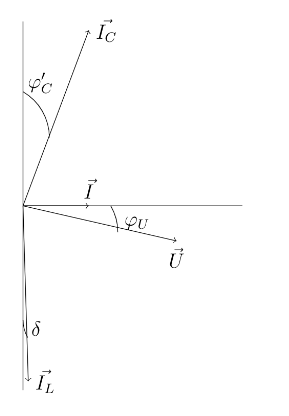
\includegraphics[width=10cm]{Screenshot from 2023-10-11 14-58-30.png}
    \caption{Векторная диаграмма токов и напряжения для контура с добротностью $Q = 17.414$}
    \label{fig:vac}
\end{figure}

% \section{Вывод}
% В ходе работы мы ознакомились с явлением резонанса токов, изучили метод комплексных амплитуд, изучили амплитудно-частотные и фазово-частотную характеристику колебательного контура, составленного из элементов, используемых в современной радиотехнике. В ходе эксперимента была с большой точностью разными методами определена добротность колебательного контура при разных значениях ёмкости конденсатора в цепи, а также рассчитаны некоторые другие характеристики контура. Результаты определения добротности непосредственными измерениями параметров контура, методом резонансных кривых и по исследованию ФЧХ совпадают. \par
% Также было исследовано само поведение токов и напряжений в контуре. Выяснено, какой вклад вносят в цепь сопротивление конденсатора (очень незначительный) и катушки (порядка сопротивления резистора в цепи). Численно получено значение индуктивности катушки и её сопротивления. Сделан вывод, что при точном расчёте цепей обязательно нужно учитывать сопротивление катушки. Была также построена векторная диаграмма токов и напряжений в исследуемом контуре, изучена природа явления резонанса токов.


\end{document}